% Gerado por scripts/gerar_tabelas.py --- não editar à mão.
\begin{figure}[htbp]
    \centering
    \caption{Risco de desligamento no ano, por tempo de casa, em 2024}
    \label{fig:risco}
    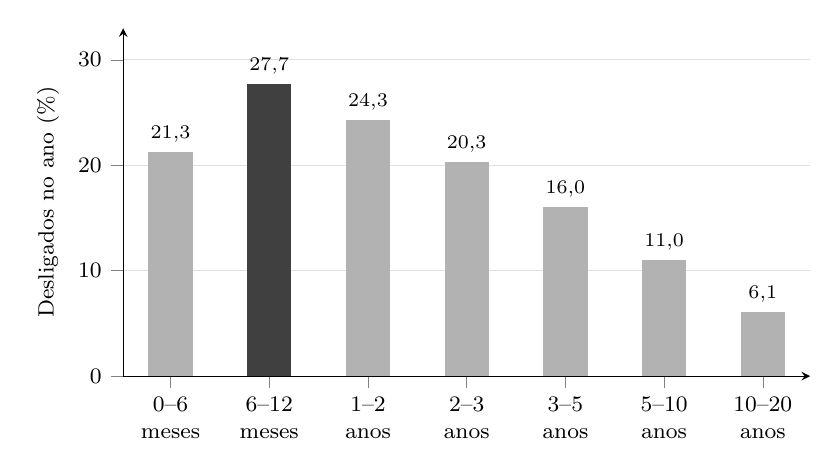
\begin{tikzpicture}
    \begin{axis}[width=\linewidth, height=6.2cm, axis lines=left, tick align=outside,
            ymajorgrids, grid style={black!12}, tick label style={font=\footnotesize},
            label style={font=\footnotesize}, title style={font=\small\bfseries},
            /pgf/number format/use comma, /pgf/number format/1000 sep={.}, width=0.85\textwidth, height=6cm, ymin=0, ymax=33,
            ylabel={Desligados no ano (\%)}, symbolic x coords={f0_6m,f6_12m,f1_2a,f2_3a,f3_5a,f5_10a,f10_20a},
            xtick={f0_6m,f6_12m,f1_2a,f2_3a,f3_5a,f5_10a,f10_20a}, xticklabels={{0--6\\meses},{6--12\\meses},{1--2\\anos},{2--3\\anos},{3--5\\anos},{5--10\\anos},{10--20\\anos}},
            enlarge x limits=0.08, ybar=0pt, bar shift=0pt,
            x tick label style={font=\footnotesize, align=center}]
        \addplot[ybar, bar width=16pt, fill=black!30, draw=none, nodes near coords, nodes near coords style={font=\scriptsize, /pgf/number format/.cd, use comma, fixed, fixed zerofill, precision=1}] coordinates {(f0_6m,21.3)};
        \addplot[ybar, bar width=16pt, fill=black!75, draw=none, nodes near coords, nodes near coords style={font=\scriptsize, /pgf/number format/.cd, use comma, fixed, fixed zerofill, precision=1}] coordinates {(f6_12m,27.7)};
        \addplot[ybar, bar width=16pt, fill=black!30, draw=none, nodes near coords, nodes near coords style={font=\scriptsize, /pgf/number format/.cd, use comma, fixed, fixed zerofill, precision=1}] coordinates {(f1_2a,24.3)};
        \addplot[ybar, bar width=16pt, fill=black!30, draw=none, nodes near coords, nodes near coords style={font=\scriptsize, /pgf/number format/.cd, use comma, fixed, fixed zerofill, precision=1}] coordinates {(f2_3a,20.3)};
        \addplot[ybar, bar width=16pt, fill=black!30, draw=none, nodes near coords, nodes near coords style={font=\scriptsize, /pgf/number format/.cd, use comma, fixed, fixed zerofill, precision=1}] coordinates {(f3_5a,16.0)};
        \addplot[ybar, bar width=16pt, fill=black!30, draw=none, nodes near coords, nodes near coords style={font=\scriptsize, /pgf/number format/.cd, use comma, fixed, fixed zerofill, precision=1}] coordinates {(f5_10a,11.0)};
        \addplot[ybar, bar width=16pt, fill=black!30, draw=none, nodes near coords, nodes near coords style={font=\scriptsize, /pgf/number format/.cd, use comma, fixed, fixed zerofill, precision=1}] coordinates {(f10_20a,6.1)};
    \end{axis}
    \end{tikzpicture}
    \\[4pt]
    {\footnotesize }Fonte: Autoria própria, a partir da camada Gold.
\end{figure}
